\section{Epoch-based Multi-commit}
\label{sec:epoch-based-multi}

% In this section we introduce the \emph{epoch-based multi-commit protocol}.
% \Cref{sec:ebmc-motivation} describes our observations and the motivation for the protocol.
% \Cref{sec:ebmc-protocol-description} presents the protocol.
% In~\Cref{sec:ebmc-fault-tolerance}, various failure scenarios are outlined.
% Finally, \Cref{sec:ebmc-discussion} discusses its limitations.
% An execution of epoch-based multi-commit is illustrated in~\Cref{fig:ebmc}.

\subsection{Rationale and Approach}
\label{sec:ebmc-motivation}

\begin{figure}[htbp]
  \centering
  \begin{tikzpicture}[node distance=2cm,scale=0.65, every node/.style={transform shape}]
    % lanes
    \draw [->,>=stealth] (1,0) -- (12,0);
    \draw [->,>=stealth] (1,-2) -- (12,-2);
    \draw [->,>=stealth] (1,-4) -- (12,-4);
    \draw [->,>=stealth] (1,-6) -- (12,-6);

    % \node (S1) at (0.4, 0) {Epoch};
    \node (C) at (0, 0  ) {Coordinator};
    \node (S2) at (0, -2) {Node $N_1$};
    \node (S3) at (0, -4) {Node $N_2$};
    \node (S4) at (0, -6) {Node $N_3$};

    \node (P) at (8, 1.5) {\small{2PC}};
    % \draw [dashed] (2,0.75) -- (11,0.75);
    \draw [dashed] (2,1.25) -- (11,1.25);
    \draw [dashed] (2,1.75) -- (11,1.75);
    \draw [dashed] (5,0.8) -- (11,0.8);

    % execution phase
    \draw [dashed] (2,1.75) -- (2,-7);
    \node (P) at (3.5, 1.5) {\small{WORK}};

    \draw [->,>=stealth] (2.4,-2.2) -- (2.6,-3.8);
    \draw [->,>=stealth] (2.8,-3.8) -- (3.0,-2.2);

    \draw [->,>=stealth] (3.3,-3.8) -- (3.5,-2.2);
    \draw [->,>=stealth] (3.7,-2.2) -- (3.9,-3.8);

    \draw [->,>=stealth] (4.2,-2.2) -- (4.4,-3.8);
    \draw [->,>=stealth] (4.6,-3.8) -- (4.8,-2.2);

    % prepare phase
    \draw [dashed] (5,1.75) -- (5,-7);
    \node (P) at (6.5, 1) {\small{PREPARE}};
    \draw [->,very thick,darkpastelblue,>=stealth] (5.2,-0.2) -- (5.6,-1.8);
    \draw [->,very thick,darkpastelblue,>=stealth] (5.2,-0.2) -- (5.8,-3.8);
    \draw [->,very thick,darkpastelblue,>=stealth] (5.2,-0.2) -- (5.8,-5.8);
    \node[draw,rectangle,minimum size=.5cm,inner sep=0pt,fill=pastelred] at (6,-2) {A};
    \node[draw,rectangle,minimum size=.5cm,inner sep=0pt,fill=pastelred] at (6.2,-4) {A};
    \node[draw,rectangle,minimum size=.5cm,inner sep=0pt,fill=pastelred] at (6.2,-6) {A};
    \draw [->,very thick,darkpastelblue,>=stealth] (7.2,-1.8) -- (7.6,-0.2);
    \draw [->,very thick,darkpastelblue,>=stealth] (7.2,-3.8) -- (7.8,-0.2);
    \draw [->,very thick,darkpastelblue,>=stealth] (7.2,-5.8) -- (7.9,-0.2);

    \node at (9.6, 0.6) {\scriptsize{$c_0=\{N_1, N_2\}, $}};
    \node at (10, 0.3) {\scriptsize{$c_1=\{N_3\}$}};

    \node at (6.6, -2.5) {\scriptsize{$dep=\{n2\}$}};
    \node at (6.6, -4.6) {\scriptsize{$dep=\{n1\}$}};
    \node at (7.2, -6.4) {\scriptsize{$dep=\{\}$}};


    % commit phase
    \draw [dashed] (8,1.25) -- (8,-7);
    \node (CO) at (9.5, 1) {\small{COMMIT}};
    \node[draw,rectangle,minimum size=.5cm,inner sep=0pt,fill=pastelred] at (8.3,0) {B};
    \draw [->,very thick,darkpastelblue,>=stealth] (8.6,-0.2) -- (9.2,-1.8);
    \draw [->,very thick,darkpastelblue,>=stealth] (8.6,-0.2) -- (9.2,-3.8);
    \draw [->,very thick,darkpastelblue,>=stealth] (8.6,-0.2) -- (9.2,-5.8);

    \draw [->,very thick,darkpastelblue,>=stealth] (10,-1.8) -- (10.6,-0.2);
    \draw [->,very thick,darkpastelblue,>=stealth] (10.2,-3.8) -- (10.8,-0.2);
    \draw [->,very thick,darkpastelblue,>=stealth] (10.4,-5.8) -- (10.9,-0.2);

    \draw [dashed] (11,1.75) -- (11,-7);

    \node[draw,circle,minimum size=.5cm,inner sep=0pt] at (4.5,-5.6) {$1$};
    \node[draw,circle,minimum size=.5cm,inner sep=0pt] at (6.3,-5.3) {$2$};
    \node[draw,circle,minimum size=.5cm,inner sep=0pt] at (9.2,-0.5) {$3$};
    \node[draw,circle,minimum size=.5cm,inner sep=0pt] at (8.4,-5.6) {$4$};
  \end{tikzpicture}
  \caption{A cycle in epoch-based multi-commit. A node's epoch-dependency list is indicated as \textit{dep}.
  %Various failure scenarios are numbered from 1 to 4.
  %Durable writes are indicated by red squares and 2PC messages by blue arrows.
  }
  \label{fig:ebmc}
\end{figure}

Epoch-based commit assumes that uncommitted data within any node is used, directly or indirectly, by every 
other node during a work interval. Hence, all transactions executed are aborted in case of a node failure.
In reality, this assumption is pessimistic and does not always hold. For example, if a node is to fail 
shortly after it starts its work interval; it would be very unlikely that each operative node executes a 
distributed transaction in that short duration
%preceding the failure
\emph{and} uses uncommitted data held by the node that goes on to fail later.

Epoch-based multi-commit avoids, where possible, aborting all transactions and thereby seeks to improve 
throughput and reduce average latency. Interactions between nodes are monitored in a lightweight, 
low-overhead manner
%. The pattern of interactions monitored is then used 
to determine whether a node needs to abort its transactions, when another node is found to have failed.
%in the 2PC cycle.
Interactions that call for aborting of transactions,  need not just be directly with the failed node but can also be transitive in nature, as explained 
%in the scenario
below.



Suppose that node $N_k$ updates an object; these updates do not become durable until $N_k$ commits and will 
be lost if $N_k$ fails before that. Let $N_j$ process a (distributed) transaction by reading an uncommitted 
update at $N_K$ and updating some local objects which are in turn read by a third $N_i$ while processing 
another transaction. If $N_k$ crashes, $N_j$ must abort its transactions as some of them involved reading 
\emph{dirty} data from $N_k$; this in turn leads to \emph{cascading aborts} at $N_i$ even though there is no 
direct interaction between $N_i$ and $N_k$.

We will express the pattern of node interactions during each work interval as a symmetric and transitive 
binary relation between nodes. This relation is called \emph{epoch dependency} and is defined as follows: 
Node $N_i$ has epoch dependency with $N_j$ during a given work interval if and only if: (i) $N_i$ accesses 
data from $N_j$ during that work interval or vice versa, or (ii) there is another $N_k$ for that work 
interval such that $N_i$ has epoch dependency with $N_k$ and $N_k$ 
%has epoch dependency
with $N_j$. 

Two remarks are in order. First, the above definition does not distinguish whether a node interaction 
involves accessing uncommitted or committed data, even though the latter does not call for cascading aborts. 
Despite some advantages in making this distinction, we avoid it in order to keep the overhead of monitoring 
node interactions as small as possible.  

Secondly, epoch dependency is also reflexive by definition, as each node accesses data from itself. So, it 
is an \emph{equivalence} relation defined on participant nodes. It therefore partitions the nodes into 
disjoint subsets which we call \emph{commit groups}: each node is in exactly one group, any two nodes of a 
group are related by epoch dependency, and no node has epoch dependency with any node not in its own group. 
Therefore, if a commit group has no failed node, then its member nodes can commit during 2PC; otherwise, they 
must abort. 

Referring to~\Cref{fig:ebmc}, we see nodes $N_1$ and $N_2$ interacting with each other during the work 
interval and $N_3$ executing no distributed transactions. So, $N_1$ and $N_2$ have epoch dependency with each 
other and $N_3$ only with itself; thus, two commit groups, $c_0 = \{N_1 , N_2 \}$ and $c_1 = \{N_3 \}$, 
emerge.
If $N_3$ fails, $N_1$ and $N_2$ can commit their transactions because they did not access any data from $N_3$.
If $N_1$ fails, $N_2 \in c_0$ must abort its transactions, while $N_3$ is unaffected.

A failed node can thus prevent nodes of only one group from committing. That is, if node interactions during 
a work interval lead to multiple commit groups emerging at the end, then all nodes do not have to abort their 
transactions in the event of a failure. On the other hand, if only one commit group exists at the end of a 
work interval, then a node failure will make all operative nodes to abort, i.e., the epoch-based multi-commit 
defaults to the original, epoch-based commit. For example, had $N_1$ and/or $N_2$ in~\Cref{fig:ebmc} 
interacted with $N_3$ during the work interval, then $c_0 = \{N_1 , N_2 , N_3 \}$ would be the only commit 
group and any node failure would mean that all other nodes aborting their transactions.

% Epoch-based multi-commit is based on the observation that not all participant
% nodes need be in the same \emph{commit group} for an epoch. % TODO: define formally
% For example, consider participant nodes 1, 2, and 3 serve transactions during an epoch.
% It is possible that node 1 and node 2 both coordinate distributed transactions that
% access data at each other, but none that access data on node 3.
% If node 3 does not coordinate any distributed transactions that access data on node 1
% or node 2,
% then a failure of node 3 need not cause node 1 and 2 to fail and unnecessarily waste
% their work.
% The relationship between participant nodes is captured by \emph{epoch dependencies}. % TODO: define formally
% If during the execution of distributed transactions, participant nodes track their epoch
% dependencies.
% At commit time, the epoch coordinator can then collects these dependencies and computes
% the set of commit groups for a given epoch.
% Only commit groups containing failed nodes need to be aborted, thus some work may be saved. 

\subsection{Motivation: TPC-C Case Study}
\label{sec:case-study:-tpc}

For multi-commit protocol to minimise
%the number of
aborts, multiple commit groups should emerge at the end of a work interval. Such an outcome depends primarily on three workload characteristics: 
(i) proportion of distributed transactions, 
(ii) average number of remote nodes accessed by distributed transactions, and
(iii) \emph{node affinity} or the likelihood of a transaction in a given node accessing data in another given node due to 
correlations between data partitions hosted by the two nodes. 

The smaller the proportion in (i), the larger is the likelihood of multiple groups. In the limit, if there are no distributed transactions at all, then each commit group is a singleton with a distinct node - as $c_1$ in~\Cref{fig:ebmc}. The smaller the average in (ii) and the stronger the affinity, the more likely is that multiple groups emerge even if the workload has a higher proportion of  distributed transactions. In what follows, we consider a canonical benchmark system  to motivate that  multi-commit scheme can be very useful in practical settings and its performance is worthy of a detailed evaluation.

% underlying data.
% To ascertain the practical utility of epoch-based multi-commit we performed a case study of a 
% realistic transactional workload, measuring the number of commit groups formed per-epoch.

TPC-C is the canonical benchmark for evaluating performance of OLTP
databases~\cite{tpcc}.
It models a warehouse order-processing application and consists of five transaction types.
Only two types, \texttt{Payment} and \texttt{NewOrder}, involve accessing remote nodes.
%; only these can introduce epoch dependencies.
%Transactions of these two types comprise 88\% of TPC-C's default workload mix.
A \texttt{Payment} transaction involves updating the payment amounts for a given
warehouse and then updating customer information.
The customer belongs to remote warehouse on another server with a 15\% probability.
In short, the \texttt{Payment} transaction accesses at most two partitions.
A \texttt{NewOrder} transaction updates 5-15 items in the stock table.
Of these items, 99\% are local to its home partition, while 1\% are at a remote partition.
%Hence, ~10\% of \texttt{NewOrder} transactions are distributed.
%Overall, the proportion of distributed transaction in the workload is 10.95\%.

\begin{figure}[htbp]
  \centering
  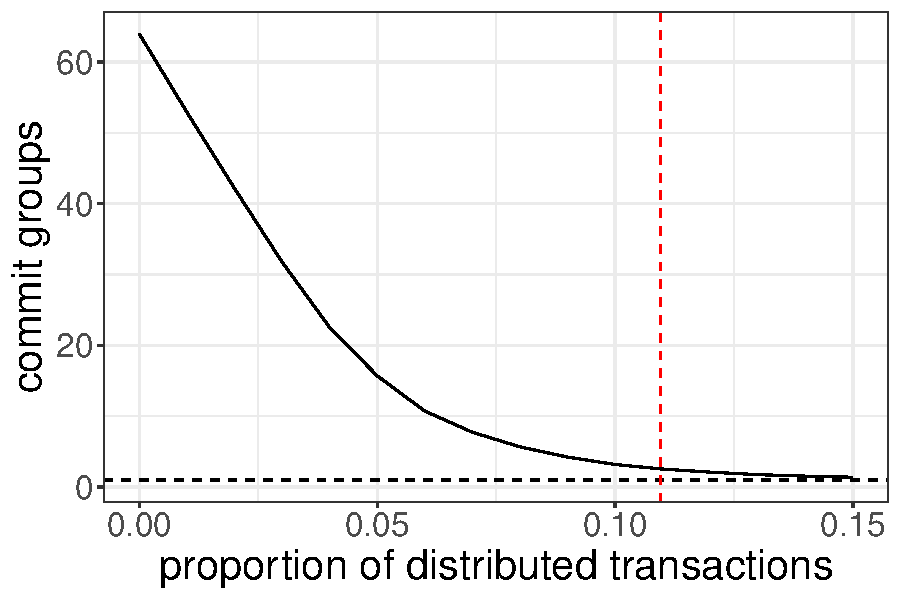
\includegraphics[width=0.6\linewidth]{figures/fig-3.pdf}
  \caption{Number of commit groups \textit{vs}  proportion of distributed transactions.
    The red line indicates the threshold after which single commit group is the only outcome.
    }
  \label{fig:3}
\end{figure}

In our experiment, the epoch size was fixed to 10$ms$ and a throughput of 300K transactions
per second in a cluster with 64 servers was assumed.
%Recall that multi-commit can be an advantage over epoch-based commit only when the numbers of commit groups emerging is
%more than 1, so that at least one  group commits in the event of a failure.
%The higher the number of commit groups formed, the more failures can be tolerated in a cycle.
\Cref{fig:3} depicts the number of commit groups formed when the the proportion of distributed transactions is varied from 1\%
to 15\%.
Commit groups are numerous when the proportion 
%of distributed transactions
does not exceed 8\% which is the typical proportion of distributed transactions encountered in practical settings. %, marginally less than the prescribed 10.95\%.
Thus, multi-commit is indeed a practical alternative to the original scheme.

\subsection{Multi-Commit Protocol Description}
\label{sec:ebmc-protocol-description}

This protocol is identical to epoch-based commit described in ~\Cref{sec:epoch-based-commit}, except for the following two additions.

\textit{Monitoring node interactions}. When node $N_i$ executes a distributed transaction and sends a \texttt{Remote-Op} message to another node $N_j$, it enters the remote $N_j$ in its local,  \textit{epoch-dependency} list. Similarly, when $N_j$ receives \texttt{Remote-Op} message from $N_i$, it enters the latter in its list. Thus, interacting nodes have each other in their \textit{epoch-dependency} lists.

\textit{Computing commit groups}. This is done by the coordinator node if some participant node has not responded to it with \texttt{Prepare-Ack} in the prepare phase of 2PC execution. Recall that the coordinator executes 2PC at the end of work interval by sending \texttt{Prepare} message to all participant nodes. (2PC messages are shown in blue in~\Cref{fig:ebmc}.) Each operative node will, in turn, respond to the coordinator by sending a \texttt{Prepare-Ack} message which will now include its epoch-dependency list as indicated in~\Cref{fig:ebmc}.

If the coordinator receives \texttt{Prepare-Ack} from all nodes, then a \texttt{Commit} message is sent to all nodes. Otherwise, it constructs a graph where a vertex represents a participant node and an edge an epoch-dependency as reported within the epoch-dependency lists it received.
Commit groups are then found by using Tarjan’s algorithm to identify strongly
connected components~\cite{tarjan}. Participant nodes of commit groups that contain no failed node are sent a \texttt{Commit} message and the rest an \texttt{Abort} message. 
 Based on the descriptions in~\cref{{sec:ebmc-motivation}}, it is easy to see that a node is sent \texttt{Commit}, if and only if it has not interacted with a failed node directly or transitively, during the work interval. (A proof by contradiction is possible and not done here.)

% hen node 1sends a \texttt{Remote-Op} message to node 2, within that message is the
% node id of sender.
% Before sending the operation it enters node 2 into its local epoch dependency list.
% When node 2 receives the \texttt{Remote-Op} message, it enters the sender's id into
% its local dependency list.

% In the absence of failures, epoch-based multi-commit produces an equivalent outcome to
% epoch-based commit.
% Differences emerge when there is a failure event in an epoch.
% In multi-commit, during the execution phase each participant node tracks epoch
% dependencies.
% An epoch dependency arises from two sources.
% Consider a distributed transaction $T$ coordinated by participant node 1.
% It happens that $T$ must access data stored on node 2.
% When node 1sends a \texttt{Remote-Op} message to node 2, within that message is the
% node id of sender.
% Before sending the operation it enters node 2 into its local epoch dependency list.
% When node 2 receives the \texttt{Remote-Op} message, it enters the sender's id into
% its local dependency list.
% Nodes 1 and 2 have now formed an bi-directional dependency between themselves,
% the outcome of their epochs is inextricably linked.
% In short, dependencies arise from the transactions a node coordinates and from
% \texttt{Remote-Op} messages they receive.

% As in~\Cref{sec:epoch-based-commit} the epoch coordinator attempts to commit the
% current epoch every $a$ milliseconds by running two phases:
% \emph{prepare} and \emph{commit}.
% Now, when a participant node receives a \texttt{Prepare} message it force logs a
% \emph{prepared write} record containing:
% (i) all transactions ids of ready-to-commit transactions,
% (ii) epoch dependencies,
% and (iii) the current epoch number, illustrated by (A) in~\Cref{fig:ebmc}.
% Then sends with a \texttt{Prepare-Ack} message to the epoch coordinator
% containing its local epoch dependencies.

% In the commit phase, the epoch coordinator collects responses from participant nodes
% and based on the received epoch dependencies computes commit groups for the epoch.
% In order to find the commit groups, the epoch coordinator represents the cluster as a
% graph, where participant nodes are represented as vertices, and epoch dependencies
% are represented as edges.
% Commit groups are then found by using Tarjan’s algorithm to identify strongly
% connected components~\cite{tarjan}.
% For each commit group,
% if any participant node fails to reply with a \texttt{Prepare-Ack} message,
% all transactions within that commit group are aborted.
% Else, the epoch coordinator force logs a \emph{commit} record with
% (i) the current epoch number, and (ii) the commit groups.
% Then, increments the global epoch, and sends \texttt{Commit} to all participant
% nodes in non-failed commit groups, illustrated by (B) in~\Cref{fig:ebmc}.
% As before, when participant nodes receives a \texttt{Commit} message it can consider
% transactions from the previous epoch committed and releases results to clients.
% They then reply with a \texttt{Commit-Ack} and prepare to begin executing transactions
% in the next epoch.

% \subsection{Fault Tolerance}
% \label{sec:ebmc-fault-tolerance}

% Again several assumptions are made:
% (i) a \emph{fail-stop} failure model,
% (ii) the epoch coordinator is implemented as a fault-tolerant replicated state machine,
% and (iii) failures are detected at the granularity of epochs.
% When a failure occurs in an epoch there are two possibilities, either the number of
% distinct commit group is equal to or larger than one.
% In the first case, behavior under node failure degrades to that described
% in~\Cref{subsec:ebc-description}.
% \Cref{fig:ebmc} presents an example of the second case.
% There are four cases to consider when a member of an operational commit group fails:
% before the epoch coordinator sends \texttt{Prepare} messages (1),
% after some member of the commit group received \texttt{Prepare} messages (2),
% after the epoch coordinator force logs the commit record (3),
% and, after some participant nodes receive \texttt{Commit} messages (4).

% %\section{Epoch-based Multi-commit}
\label{sec:epoch-based-multi}

% In this section we introduce the \emph{epoch-based multi-commit protocol}.
% \Cref{sec:ebmc-motivation} describes our observations and the motivation for the protocol.
% \Cref{sec:ebmc-protocol-description} presents the protocol.
% In~\Cref{sec:ebmc-fault-tolerance}, various failure scenarios are outlined.
% Finally, \Cref{sec:ebmc-discussion} discusses its limitations.
% An execution of epoch-based multi-commit is illustrated in~\Cref{fig:ebmc}.

\subsection{Rationale and Approach}
\label{sec:ebmc-motivation}

\begin{figure}[htbp]
  \centering
  \begin{tikzpicture}[node distance=2cm,scale=0.65, every node/.style={transform shape}]
    % lanes
    \draw [->,>=stealth] (1,0) -- (12,0);
    \draw [->,>=stealth] (1,-2) -- (12,-2);
    \draw [->,>=stealth] (1,-4) -- (12,-4);
    \draw [->,>=stealth] (1,-6) -- (12,-6);

    % \node (S1) at (0.4, 0) {Epoch};
    \node (C) at (0, 0  ) {Coordinator};
    \node (S2) at (0, -2) {Node $N_1$};
    \node (S3) at (0, -4) {Node $N_2$};
    \node (S4) at (0, -6) {Node $N_3$};

    \node (P) at (8, 1.5) {\small{2PC}};
    % \draw [dashed] (2,0.75) -- (11,0.75);
    \draw [dashed] (2,1.25) -- (11,1.25);
    \draw [dashed] (2,1.75) -- (11,1.75);
    \draw [dashed] (5,0.8) -- (11,0.8);

    % execution phase
    \draw [dashed] (2,1.75) -- (2,-7);
    \node (P) at (3.5, 1.5) {\small{WORK}};

    \draw [->,>=stealth] (2.4,-2.2) -- (2.6,-3.8);
    \draw [->,>=stealth] (2.8,-3.8) -- (3.0,-2.2);

    \draw [->,>=stealth] (3.3,-3.8) -- (3.5,-2.2);
    \draw [->,>=stealth] (3.7,-2.2) -- (3.9,-3.8);

    \draw [->,>=stealth] (4.2,-2.2) -- (4.4,-3.8);
    \draw [->,>=stealth] (4.6,-3.8) -- (4.8,-2.2);

    % prepare phase
    \draw [dashed] (5,1.75) -- (5,-7);
    \node (P) at (6.5, 1) {\small{PREPARE}};
    \draw [->,very thick,darkpastelblue,>=stealth] (5.2,-0.2) -- (5.6,-1.8);
    \draw [->,very thick,darkpastelblue,>=stealth] (5.2,-0.2) -- (5.8,-3.8);
    \draw [->,very thick,darkpastelblue,>=stealth] (5.2,-0.2) -- (5.8,-5.8);
    \node[draw,rectangle,minimum size=.5cm,inner sep=0pt,fill=pastelred] at (6,-2) {A};
    \node[draw,rectangle,minimum size=.5cm,inner sep=0pt,fill=pastelred] at (6.2,-4) {A};
    \node[draw,rectangle,minimum size=.5cm,inner sep=0pt,fill=pastelred] at (6.2,-6) {A};
    \draw [->,very thick,darkpastelblue,>=stealth] (7.2,-1.8) -- (7.6,-0.2);
    \draw [->,very thick,darkpastelblue,>=stealth] (7.2,-3.8) -- (7.8,-0.2);
    \draw [->,very thick,darkpastelblue,>=stealth] (7.2,-5.8) -- (7.9,-0.2);

    \node at (9.6, 0.6) {\scriptsize{$c_0=\{N_1, N_2\}, $}};
    \node at (10, 0.3) {\scriptsize{$c_1=\{N_3\}$}};

    \node at (6.6, -2.5) {\scriptsize{$dep=\{n2\}$}};
    \node at (6.6, -4.6) {\scriptsize{$dep=\{n1\}$}};
    \node at (7.2, -6.4) {\scriptsize{$dep=\{\}$}};


    % commit phase
    \draw [dashed] (8,1.25) -- (8,-7);
    \node (CO) at (9.5, 1) {\small{COMMIT}};
    \node[draw,rectangle,minimum size=.5cm,inner sep=0pt,fill=pastelred] at (8.3,0) {B};
    \draw [->,very thick,darkpastelblue,>=stealth] (8.6,-0.2) -- (9.2,-1.8);
    \draw [->,very thick,darkpastelblue,>=stealth] (8.6,-0.2) -- (9.2,-3.8);
    \draw [->,very thick,darkpastelblue,>=stealth] (8.6,-0.2) -- (9.2,-5.8);

    \draw [->,very thick,darkpastelblue,>=stealth] (10,-1.8) -- (10.6,-0.2);
    \draw [->,very thick,darkpastelblue,>=stealth] (10.2,-3.8) -- (10.8,-0.2);
    \draw [->,very thick,darkpastelblue,>=stealth] (10.4,-5.8) -- (10.9,-0.2);

    \draw [dashed] (11,1.75) -- (11,-7);

    \node[draw,circle,minimum size=.5cm,inner sep=0pt] at (4.5,-5.6) {$1$};
    \node[draw,circle,minimum size=.5cm,inner sep=0pt] at (6.3,-5.3) {$2$};
    \node[draw,circle,minimum size=.5cm,inner sep=0pt] at (9.2,-0.5) {$3$};
    \node[draw,circle,minimum size=.5cm,inner sep=0pt] at (8.4,-5.6) {$4$};
  \end{tikzpicture}
  \caption{A cycle in epoch-based multi-commit. A node's epoch-dependency list is indicated as \textit{dep}.
  %Various failure scenarios are numbered from 1 to 4.
  %Durable writes are indicated by red squares and 2PC messages by blue arrows.
  }
  \label{fig:ebmc}
\end{figure}

Epoch-based commit assumes that uncommitted data within any node is used, directly or indirectly, by every 
other node during a work interval. Hence, all transactions executed are aborted in case of a node failure.
In reality, this assumption is pessimistic and does not always hold. For example, if a node is to fail 
shortly after it starts its work interval; it would be very unlikely that each operative node executes a 
distributed transaction in that short duration
%preceding the failure
\emph{and} uses uncommitted data held by the node that goes on to fail later.

Epoch-based multi-commit avoids, where possible, aborting all transactions and thereby seeks to improve 
throughput and reduce average latency. Interactions between nodes are monitored in a lightweight, 
low-overhead manner
%. The pattern of interactions monitored is then used 
to determine whether a node needs to abort its transactions, when another node is found to have failed.
%in the 2PC cycle.
Interactions that call for aborting of transactions,  need not just be directly with the failed node but can also be transitive in nature, as explained 
%in the scenario
below.



Suppose that node $N_k$ updates an object; these updates do not become durable until $N_k$ commits and will 
be lost if $N_k$ fails before that. Let $N_j$ process a (distributed) transaction by reading an uncommitted 
update at $N_K$ and updating some local objects which are in turn read by a third $N_i$ while processing 
another transaction. If $N_k$ crashes, $N_j$ must abort its transactions as some of them involved reading 
\emph{dirty} data from $N_k$; this in turn leads to \emph{cascading aborts} at $N_i$ even though there is no 
direct interaction between $N_i$ and $N_k$.

We will express the pattern of node interactions during each work interval as a symmetric and transitive 
binary relation between nodes. This relation is called \emph{epoch dependency} and is defined as follows: 
Node $N_i$ has epoch dependency with $N_j$ during a given work interval if and only if: (i) $N_i$ accesses 
data from $N_j$ during that work interval or vice versa, or (ii) there is another $N_k$ for that work 
interval such that $N_i$ has epoch dependency with $N_k$ and $N_k$ 
%has epoch dependency
with $N_j$. 

Two remarks are in order. First, the above definition does not distinguish whether a node interaction 
involves accessing uncommitted or committed data, even though the latter does not call for cascading aborts. 
Despite some advantages in making this distinction, we avoid it in order to keep the overhead of monitoring 
node interactions as small as possible.  

Secondly, epoch dependency is also reflexive by definition, as each node accesses data from itself. So, it 
is an \emph{equivalence} relation defined on participant nodes. It therefore partitions the nodes into 
disjoint subsets which we call \emph{commit groups}: each node is in exactly one group, any two nodes of a 
group are related by epoch dependency, and no node has epoch dependency with any node not in its own group. 
Therefore, if a commit group has no failed node, then its member nodes can commit during 2PC; otherwise, they 
must abort. 

Referring to~\Cref{fig:ebmc}, we see nodes $N_1$ and $N_2$ interacting with each other during the work 
interval and $N_3$ executing no distributed transactions. So, $N_1$ and $N_2$ have epoch dependency with each 
other and $N_3$ only with itself; thus, two commit groups, $c_0 = \{N_1 , N_2 \}$ and $c_1 = \{N_3 \}$, 
emerge.
If $N_3$ fails, $N_1$ and $N_2$ can commit their transactions because they did not access any data from $N_3$.
If $N_1$ fails, $N_2 \in c_0$ must abort its transactions, while $N_3$ is unaffected.

A failed node can thus prevent nodes of only one group from committing. That is, if node interactions during 
a work interval lead to multiple commit groups emerging at the end, then all nodes do not have to abort their 
transactions in the event of a failure. On the other hand, if only one commit group exists at the end of a 
work interval, then a node failure will make all operative nodes to abort, i.e., the epoch-based multi-commit 
defaults to the original, epoch-based commit. For example, had $N_1$ and/or $N_2$ in~\Cref{fig:ebmc} 
interacted with $N_3$ during the work interval, then $c_0 = \{N_1 , N_2 , N_3 \}$ would be the only commit 
group and any node failure would mean that all other nodes aborting their transactions.

% Epoch-based multi-commit is based on the observation that not all participant
% nodes need be in the same \emph{commit group} for an epoch. % TODO: define formally
% For example, consider participant nodes 1, 2, and 3 serve transactions during an epoch.
% It is possible that node 1 and node 2 both coordinate distributed transactions that
% access data at each other, but none that access data on node 3.
% If node 3 does not coordinate any distributed transactions that access data on node 1
% or node 2,
% then a failure of node 3 need not cause node 1 and 2 to fail and unnecessarily waste
% their work.
% The relationship between participant nodes is captured by \emph{epoch dependencies}. % TODO: define formally
% If during the execution of distributed transactions, participant nodes track their epoch
% dependencies.
% At commit time, the epoch coordinator can then collects these dependencies and computes
% the set of commit groups for a given epoch.
% Only commit groups containing failed nodes need to be aborted, thus some work may be saved. 

\subsection{Motivation: TPC-C Case Study}
\label{sec:case-study:-tpc}

For multi-commit protocol to minimise
%the number of
aborts, multiple commit groups should emerge at the end of a work interval. Such an outcome depends primarily on three workload characteristics: 
(i) proportion of distributed transactions, 
(ii) average number of remote nodes accessed by distributed transactions, and
(iii) \emph{node affinity} or the likelihood of a transaction in a given node accessing data in another given node due to 
correlations between data partitions hosted by the two nodes. 

The smaller the proportion in (i), the larger is the likelihood of multiple groups. In the limit, if there are no distributed transactions at all, then each commit group is a singleton with a distinct node - as $c_1$ in~\Cref{fig:ebmc}. The smaller the average in (ii) and the stronger the affinity, the more likely is that multiple groups emerge even if the workload has a higher proportion of  distributed transactions. In what follows, we consider a canonical benchmark system  to motivate that  multi-commit scheme can be very useful in practical settings and its performance is worthy of a detailed evaluation.

% underlying data.
% To ascertain the practical utility of epoch-based multi-commit we performed a case study of a 
% realistic transactional workload, measuring the number of commit groups formed per-epoch.

TPC-C is the canonical benchmark for evaluating performance of OLTP
databases~\cite{tpcc}.
It models a warehouse order-processing application and consists of five transaction types.
Only two types, \texttt{Payment} and \texttt{NewOrder}, involve accessing remote nodes.
%; only these can introduce epoch dependencies.
%Transactions of these two types comprise 88\% of TPC-C's default workload mix.
A \texttt{Payment} transaction involves updating the payment amounts for a given
warehouse and then updating customer information.
The customer belongs to remote warehouse on another server with a 15\% probability.
In short, the \texttt{Payment} transaction accesses at most two partitions.
A \texttt{NewOrder} transaction updates 5-15 items in the stock table.
Of these items, 99\% are local to its home partition, while 1\% are at a remote partition.
%Hence, ~10\% of \texttt{NewOrder} transactions are distributed.
%Overall, the proportion of distributed transaction in the workload is 10.95\%.

\begin{figure}[htbp]
  \centering
  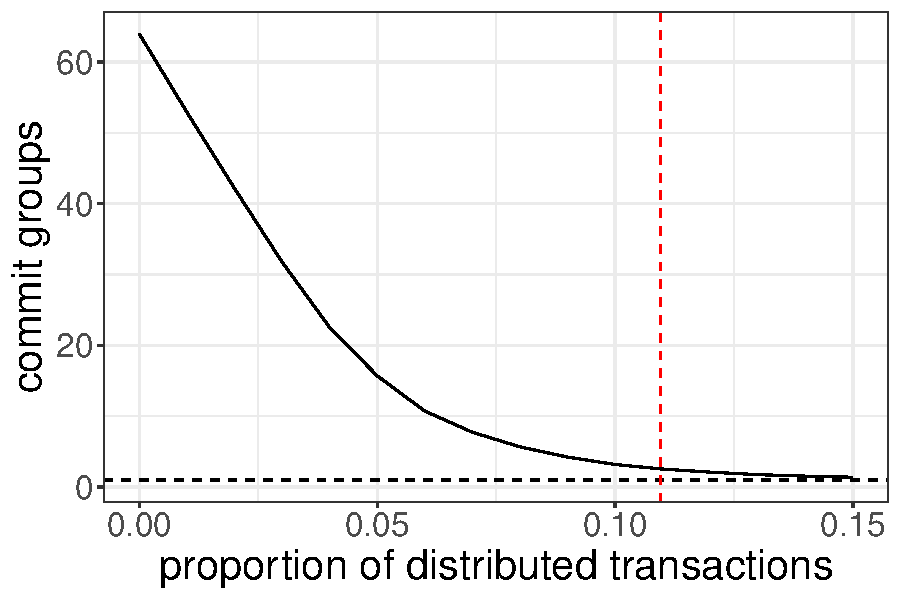
\includegraphics[width=0.6\linewidth]{figures/fig-3.pdf}
  \caption{Number of commit groups \textit{vs}  proportion of distributed transactions.
    The red line indicates the threshold after which single commit group is the only outcome.
    }
  \label{fig:3}
\end{figure}

In our experiment, the epoch size was fixed to 10$ms$ and a throughput of 300K transactions
per second in a cluster with 64 servers was assumed.
%Recall that multi-commit can be an advantage over epoch-based commit only when the numbers of commit groups emerging is
%more than 1, so that at least one  group commits in the event of a failure.
%The higher the number of commit groups formed, the more failures can be tolerated in a cycle.
\Cref{fig:3} depicts the number of commit groups formed when the the proportion of distributed transactions is varied from 1\%
to 15\%.
Commit groups are numerous when the proportion 
%of distributed transactions
does not exceed 8\% which is the typical proportion of distributed transactions encountered in practical settings. %, marginally less than the prescribed 10.95\%.
Thus, multi-commit is indeed a practical alternative to the original scheme.

\subsection{Multi-Commit Protocol Description}
\label{sec:ebmc-protocol-description}

This protocol is identical to epoch-based commit described in ~\Cref{sec:epoch-based-commit}, except for the following two additions.

\textit{Monitoring node interactions}. When node $N_i$ executes a distributed transaction and sends a \texttt{Remote-Op} message to another node $N_j$, it enters the remote $N_j$ in its local,  \textit{epoch-dependency} list. Similarly, when $N_j$ receives \texttt{Remote-Op} message from $N_i$, it enters the latter in its list. Thus, interacting nodes have each other in their \textit{epoch-dependency} lists.

\textit{Computing commit groups}. This is done by the coordinator node if some participant node has not responded to it with \texttt{Prepare-Ack} in the prepare phase of 2PC execution. Recall that the coordinator executes 2PC at the end of work interval by sending \texttt{Prepare} message to all participant nodes. (2PC messages are shown in blue in~\Cref{fig:ebmc}.) Each operative node will, in turn, respond to the coordinator by sending a \texttt{Prepare-Ack} message which will now include its epoch-dependency list as indicated in~\Cref{fig:ebmc}.

If the coordinator receives \texttt{Prepare-Ack} from all nodes, then a \texttt{Commit} message is sent to all nodes. Otherwise, it constructs a graph where a vertex represents a participant node and an edge an epoch-dependency as reported within the epoch-dependency lists it received.
Commit groups are then found by using Tarjan’s algorithm to identify strongly
connected components~\cite{tarjan}. Participant nodes of commit groups that contain no failed node are sent a \texttt{Commit} message and the rest an \texttt{Abort} message. 
 Based on the descriptions in~\cref{{sec:ebmc-motivation}}, it is easy to see that a node is sent \texttt{Commit}, if and only if it has not interacted with a failed node directly or transitively, during the work interval. (A proof by contradiction is possible and not done here.)

% hen node 1sends a \texttt{Remote-Op} message to node 2, within that message is the
% node id of sender.
% Before sending the operation it enters node 2 into its local epoch dependency list.
% When node 2 receives the \texttt{Remote-Op} message, it enters the sender's id into
% its local dependency list.

% In the absence of failures, epoch-based multi-commit produces an equivalent outcome to
% epoch-based commit.
% Differences emerge when there is a failure event in an epoch.
% In multi-commit, during the execution phase each participant node tracks epoch
% dependencies.
% An epoch dependency arises from two sources.
% Consider a distributed transaction $T$ coordinated by participant node 1.
% It happens that $T$ must access data stored on node 2.
% When node 1sends a \texttt{Remote-Op} message to node 2, within that message is the
% node id of sender.
% Before sending the operation it enters node 2 into its local epoch dependency list.
% When node 2 receives the \texttt{Remote-Op} message, it enters the sender's id into
% its local dependency list.
% Nodes 1 and 2 have now formed an bi-directional dependency between themselves,
% the outcome of their epochs is inextricably linked.
% In short, dependencies arise from the transactions a node coordinates and from
% \texttt{Remote-Op} messages they receive.

% As in~\Cref{sec:epoch-based-commit} the epoch coordinator attempts to commit the
% current epoch every $a$ milliseconds by running two phases:
% \emph{prepare} and \emph{commit}.
% Now, when a participant node receives a \texttt{Prepare} message it force logs a
% \emph{prepared write} record containing:
% (i) all transactions ids of ready-to-commit transactions,
% (ii) epoch dependencies,
% and (iii) the current epoch number, illustrated by (A) in~\Cref{fig:ebmc}.
% Then sends with a \texttt{Prepare-Ack} message to the epoch coordinator
% containing its local epoch dependencies.

% In the commit phase, the epoch coordinator collects responses from participant nodes
% and based on the received epoch dependencies computes commit groups for the epoch.
% In order to find the commit groups, the epoch coordinator represents the cluster as a
% graph, where participant nodes are represented as vertices, and epoch dependencies
% are represented as edges.
% Commit groups are then found by using Tarjan’s algorithm to identify strongly
% connected components~\cite{tarjan}.
% For each commit group,
% if any participant node fails to reply with a \texttt{Prepare-Ack} message,
% all transactions within that commit group are aborted.
% Else, the epoch coordinator force logs a \emph{commit} record with
% (i) the current epoch number, and (ii) the commit groups.
% Then, increments the global epoch, and sends \texttt{Commit} to all participant
% nodes in non-failed commit groups, illustrated by (B) in~\Cref{fig:ebmc}.
% As before, when participant nodes receives a \texttt{Commit} message it can consider
% transactions from the previous epoch committed and releases results to clients.
% They then reply with a \texttt{Commit-Ack} and prepare to begin executing transactions
% in the next epoch.

% \subsection{Fault Tolerance}
% \label{sec:ebmc-fault-tolerance}

% Again several assumptions are made:
% (i) a \emph{fail-stop} failure model,
% (ii) the epoch coordinator is implemented as a fault-tolerant replicated state machine,
% and (iii) failures are detected at the granularity of epochs.
% When a failure occurs in an epoch there are two possibilities, either the number of
% distinct commit group is equal to or larger than one.
% In the first case, behavior under node failure degrades to that described
% in~\Cref{subsec:ebc-description}.
% \Cref{fig:ebmc} presents an example of the second case.
% There are four cases to consider when a member of an operational commit group fails:
% before the epoch coordinator sends \texttt{Prepare} messages (1),
% after some member of the commit group received \texttt{Prepare} messages (2),
% after the epoch coordinator force logs the commit record (3),
% and, after some participant nodes receive \texttt{Commit} messages (4).

% %\section{Epoch-based Multi-commit}
\label{sec:epoch-based-multi}

% In this section we introduce the \emph{epoch-based multi-commit protocol}.
% \Cref{sec:ebmc-motivation} describes our observations and the motivation for the protocol.
% \Cref{sec:ebmc-protocol-description} presents the protocol.
% In~\Cref{sec:ebmc-fault-tolerance}, various failure scenarios are outlined.
% Finally, \Cref{sec:ebmc-discussion} discusses its limitations.
% An execution of epoch-based multi-commit is illustrated in~\Cref{fig:ebmc}.

\subsection{Rationale and Approach}
\label{sec:ebmc-motivation}

\begin{figure}[htbp]
  \centering
  \begin{tikzpicture}[node distance=2cm,scale=0.65, every node/.style={transform shape}]
    % lanes
    \draw [->,>=stealth] (1,0) -- (12,0);
    \draw [->,>=stealth] (1,-2) -- (12,-2);
    \draw [->,>=stealth] (1,-4) -- (12,-4);
    \draw [->,>=stealth] (1,-6) -- (12,-6);

    % \node (S1) at (0.4, 0) {Epoch};
    \node (C) at (0, 0  ) {Coordinator};
    \node (S2) at (0, -2) {Node $N_1$};
    \node (S3) at (0, -4) {Node $N_2$};
    \node (S4) at (0, -6) {Node $N_3$};

    \node (P) at (8, 1.5) {\small{2PC}};
    % \draw [dashed] (2,0.75) -- (11,0.75);
    \draw [dashed] (2,1.25) -- (11,1.25);
    \draw [dashed] (2,1.75) -- (11,1.75);
    \draw [dashed] (5,0.8) -- (11,0.8);

    % execution phase
    \draw [dashed] (2,1.75) -- (2,-7);
    \node (P) at (3.5, 1.5) {\small{WORK}};

    \draw [->,>=stealth] (2.4,-2.2) -- (2.6,-3.8);
    \draw [->,>=stealth] (2.8,-3.8) -- (3.0,-2.2);

    \draw [->,>=stealth] (3.3,-3.8) -- (3.5,-2.2);
    \draw [->,>=stealth] (3.7,-2.2) -- (3.9,-3.8);

    \draw [->,>=stealth] (4.2,-2.2) -- (4.4,-3.8);
    \draw [->,>=stealth] (4.6,-3.8) -- (4.8,-2.2);

    % prepare phase
    \draw [dashed] (5,1.75) -- (5,-7);
    \node (P) at (6.5, 1) {\small{PREPARE}};
    \draw [->,very thick,darkpastelblue,>=stealth] (5.2,-0.2) -- (5.6,-1.8);
    \draw [->,very thick,darkpastelblue,>=stealth] (5.2,-0.2) -- (5.8,-3.8);
    \draw [->,very thick,darkpastelblue,>=stealth] (5.2,-0.2) -- (5.8,-5.8);
    \node[draw,rectangle,minimum size=.5cm,inner sep=0pt,fill=pastelred] at (6,-2) {A};
    \node[draw,rectangle,minimum size=.5cm,inner sep=0pt,fill=pastelred] at (6.2,-4) {A};
    \node[draw,rectangle,minimum size=.5cm,inner sep=0pt,fill=pastelred] at (6.2,-6) {A};
    \draw [->,very thick,darkpastelblue,>=stealth] (7.2,-1.8) -- (7.6,-0.2);
    \draw [->,very thick,darkpastelblue,>=stealth] (7.2,-3.8) -- (7.8,-0.2);
    \draw [->,very thick,darkpastelblue,>=stealth] (7.2,-5.8) -- (7.9,-0.2);

    \node at (9.6, 0.6) {\scriptsize{$c_0=\{N_1, N_2\}, $}};
    \node at (10, 0.3) {\scriptsize{$c_1=\{N_3\}$}};

    \node at (6.6, -2.5) {\scriptsize{$dep=\{n2\}$}};
    \node at (6.6, -4.6) {\scriptsize{$dep=\{n1\}$}};
    \node at (7.2, -6.4) {\scriptsize{$dep=\{\}$}};


    % commit phase
    \draw [dashed] (8,1.25) -- (8,-7);
    \node (CO) at (9.5, 1) {\small{COMMIT}};
    \node[draw,rectangle,minimum size=.5cm,inner sep=0pt,fill=pastelred] at (8.3,0) {B};
    \draw [->,very thick,darkpastelblue,>=stealth] (8.6,-0.2) -- (9.2,-1.8);
    \draw [->,very thick,darkpastelblue,>=stealth] (8.6,-0.2) -- (9.2,-3.8);
    \draw [->,very thick,darkpastelblue,>=stealth] (8.6,-0.2) -- (9.2,-5.8);

    \draw [->,very thick,darkpastelblue,>=stealth] (10,-1.8) -- (10.6,-0.2);
    \draw [->,very thick,darkpastelblue,>=stealth] (10.2,-3.8) -- (10.8,-0.2);
    \draw [->,very thick,darkpastelblue,>=stealth] (10.4,-5.8) -- (10.9,-0.2);

    \draw [dashed] (11,1.75) -- (11,-7);

    \node[draw,circle,minimum size=.5cm,inner sep=0pt] at (4.5,-5.6) {$1$};
    \node[draw,circle,minimum size=.5cm,inner sep=0pt] at (6.3,-5.3) {$2$};
    \node[draw,circle,minimum size=.5cm,inner sep=0pt] at (9.2,-0.5) {$3$};
    \node[draw,circle,minimum size=.5cm,inner sep=0pt] at (8.4,-5.6) {$4$};
  \end{tikzpicture}
  \caption{A cycle in epoch-based multi-commit. A node's epoch-dependency list is indicated as \textit{dep}.
  %Various failure scenarios are numbered from 1 to 4.
  %Durable writes are indicated by red squares and 2PC messages by blue arrows.
  }
  \label{fig:ebmc}
\end{figure}

Epoch-based commit assumes that uncommitted data within any node is used, directly or indirectly, by every 
other node during a work interval. Hence, all transactions executed are aborted in case of a node failure.
In reality, this assumption is pessimistic and does not always hold. For example, if a node is to fail 
shortly after it starts its work interval; it would be very unlikely that each operative node executes a 
distributed transaction in that short duration
%preceding the failure
\emph{and} uses uncommitted data held by the node that goes on to fail later.

Epoch-based multi-commit avoids, where possible, aborting all transactions and thereby seeks to improve 
throughput and reduce average latency. Interactions between nodes are monitored in a lightweight, 
low-overhead manner
%. The pattern of interactions monitored is then used 
to determine whether a node needs to abort its transactions, when another node is found to have failed.
%in the 2PC cycle.
Interactions that call for aborting of transactions,  need not just be directly with the failed node but can also be transitive in nature, as explained 
%in the scenario
below.



Suppose that node $N_k$ updates an object; these updates do not become durable until $N_k$ commits and will 
be lost if $N_k$ fails before that. Let $N_j$ process a (distributed) transaction by reading an uncommitted 
update at $N_K$ and updating some local objects which are in turn read by a third $N_i$ while processing 
another transaction. If $N_k$ crashes, $N_j$ must abort its transactions as some of them involved reading 
\emph{dirty} data from $N_k$; this in turn leads to \emph{cascading aborts} at $N_i$ even though there is no 
direct interaction between $N_i$ and $N_k$.

We will express the pattern of node interactions during each work interval as a symmetric and transitive 
binary relation between nodes. This relation is called \emph{epoch dependency} and is defined as follows: 
Node $N_i$ has epoch dependency with $N_j$ during a given work interval if and only if: (i) $N_i$ accesses 
data from $N_j$ during that work interval or vice versa, or (ii) there is another $N_k$ for that work 
interval such that $N_i$ has epoch dependency with $N_k$ and $N_k$ 
%has epoch dependency
with $N_j$. 

Two remarks are in order. First, the above definition does not distinguish whether a node interaction 
involves accessing uncommitted or committed data, even though the latter does not call for cascading aborts. 
Despite some advantages in making this distinction, we avoid it in order to keep the overhead of monitoring 
node interactions as small as possible.  

Secondly, epoch dependency is also reflexive by definition, as each node accesses data from itself. So, it 
is an \emph{equivalence} relation defined on participant nodes. It therefore partitions the nodes into 
disjoint subsets which we call \emph{commit groups}: each node is in exactly one group, any two nodes of a 
group are related by epoch dependency, and no node has epoch dependency with any node not in its own group. 
Therefore, if a commit group has no failed node, then its member nodes can commit during 2PC; otherwise, they 
must abort. 

Referring to~\Cref{fig:ebmc}, we see nodes $N_1$ and $N_2$ interacting with each other during the work 
interval and $N_3$ executing no distributed transactions. So, $N_1$ and $N_2$ have epoch dependency with each 
other and $N_3$ only with itself; thus, two commit groups, $c_0 = \{N_1 , N_2 \}$ and $c_1 = \{N_3 \}$, 
emerge.
If $N_3$ fails, $N_1$ and $N_2$ can commit their transactions because they did not access any data from $N_3$.
If $N_1$ fails, $N_2 \in c_0$ must abort its transactions, while $N_3$ is unaffected.

A failed node can thus prevent nodes of only one group from committing. That is, if node interactions during 
a work interval lead to multiple commit groups emerging at the end, then all nodes do not have to abort their 
transactions in the event of a failure. On the other hand, if only one commit group exists at the end of a 
work interval, then a node failure will make all operative nodes to abort, i.e., the epoch-based multi-commit 
defaults to the original, epoch-based commit. For example, had $N_1$ and/or $N_2$ in~\Cref{fig:ebmc} 
interacted with $N_3$ during the work interval, then $c_0 = \{N_1 , N_2 , N_3 \}$ would be the only commit 
group and any node failure would mean that all other nodes aborting their transactions.

% Epoch-based multi-commit is based on the observation that not all participant
% nodes need be in the same \emph{commit group} for an epoch. % TODO: define formally
% For example, consider participant nodes 1, 2, and 3 serve transactions during an epoch.
% It is possible that node 1 and node 2 both coordinate distributed transactions that
% access data at each other, but none that access data on node 3.
% If node 3 does not coordinate any distributed transactions that access data on node 1
% or node 2,
% then a failure of node 3 need not cause node 1 and 2 to fail and unnecessarily waste
% their work.
% The relationship between participant nodes is captured by \emph{epoch dependencies}. % TODO: define formally
% If during the execution of distributed transactions, participant nodes track their epoch
% dependencies.
% At commit time, the epoch coordinator can then collects these dependencies and computes
% the set of commit groups for a given epoch.
% Only commit groups containing failed nodes need to be aborted, thus some work may be saved. 

\subsection{Motivation: TPC-C Case Study}
\label{sec:case-study:-tpc}

For multi-commit protocol to minimise
%the number of
aborts, multiple commit groups should emerge at the end of a work interval. Such an outcome depends primarily on three workload characteristics: 
(i) proportion of distributed transactions, 
(ii) average number of remote nodes accessed by distributed transactions, and
(iii) \emph{node affinity} or the likelihood of a transaction in a given node accessing data in another given node due to 
correlations between data partitions hosted by the two nodes. 

The smaller the proportion in (i), the larger is the likelihood of multiple groups. In the limit, if there are no distributed transactions at all, then each commit group is a singleton with a distinct node - as $c_1$ in~\Cref{fig:ebmc}. The smaller the average in (ii) and the stronger the affinity, the more likely is that multiple groups emerge even if the workload has a higher proportion of  distributed transactions. In what follows, we consider a canonical benchmark system  to motivate that  multi-commit scheme can be very useful in practical settings and its performance is worthy of a detailed evaluation.

% underlying data.
% To ascertain the practical utility of epoch-based multi-commit we performed a case study of a 
% realistic transactional workload, measuring the number of commit groups formed per-epoch.

TPC-C is the canonical benchmark for evaluating performance of OLTP
databases~\cite{tpcc}.
It models a warehouse order-processing application and consists of five transaction types.
Only two types, \texttt{Payment} and \texttt{NewOrder}, involve accessing remote nodes.
%; only these can introduce epoch dependencies.
%Transactions of these two types comprise 88\% of TPC-C's default workload mix.
A \texttt{Payment} transaction involves updating the payment amounts for a given
warehouse and then updating customer information.
The customer belongs to remote warehouse on another server with a 15\% probability.
In short, the \texttt{Payment} transaction accesses at most two partitions.
A \texttt{NewOrder} transaction updates 5-15 items in the stock table.
Of these items, 99\% are local to its home partition, while 1\% are at a remote partition.
%Hence, ~10\% of \texttt{NewOrder} transactions are distributed.
%Overall, the proportion of distributed transaction in the workload is 10.95\%.

\begin{figure}[htbp]
  \centering
  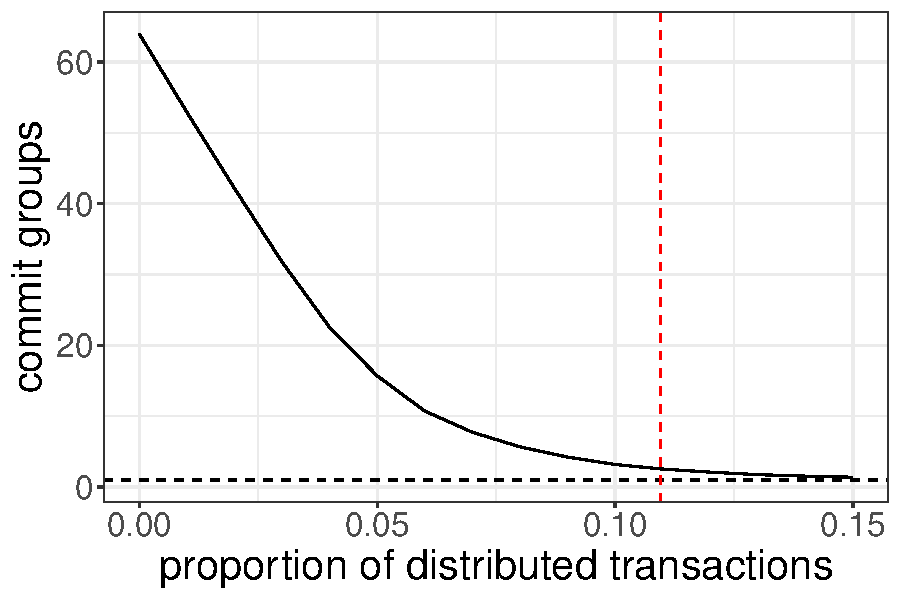
\includegraphics[width=0.6\linewidth]{figures/fig-3.pdf}
  \caption{Number of commit groups \textit{vs}  proportion of distributed transactions.
    The red line indicates the threshold after which single commit group is the only outcome.
    }
  \label{fig:3}
\end{figure}

In our experiment, the epoch size was fixed to 10$ms$ and a throughput of 300K transactions
per second in a cluster with 64 servers was assumed.
%Recall that multi-commit can be an advantage over epoch-based commit only when the numbers of commit groups emerging is
%more than 1, so that at least one  group commits in the event of a failure.
%The higher the number of commit groups formed, the more failures can be tolerated in a cycle.
\Cref{fig:3} depicts the number of commit groups formed when the the proportion of distributed transactions is varied from 1\%
to 15\%.
Commit groups are numerous when the proportion 
%of distributed transactions
does not exceed 8\% which is the typical proportion of distributed transactions encountered in practical settings. %, marginally less than the prescribed 10.95\%.
Thus, multi-commit is indeed a practical alternative to the original scheme.

\subsection{Multi-Commit Protocol Description}
\label{sec:ebmc-protocol-description}

This protocol is identical to epoch-based commit described in ~\Cref{sec:epoch-based-commit}, except for the following two additions.

\textit{Monitoring node interactions}. When node $N_i$ executes a distributed transaction and sends a \texttt{Remote-Op} message to another node $N_j$, it enters the remote $N_j$ in its local,  \textit{epoch-dependency} list. Similarly, when $N_j$ receives \texttt{Remote-Op} message from $N_i$, it enters the latter in its list. Thus, interacting nodes have each other in their \textit{epoch-dependency} lists.

\textit{Computing commit groups}. This is done by the coordinator node if some participant node has not responded to it with \texttt{Prepare-Ack} in the prepare phase of 2PC execution. Recall that the coordinator executes 2PC at the end of work interval by sending \texttt{Prepare} message to all participant nodes. (2PC messages are shown in blue in~\Cref{fig:ebmc}.) Each operative node will, in turn, respond to the coordinator by sending a \texttt{Prepare-Ack} message which will now include its epoch-dependency list as indicated in~\Cref{fig:ebmc}.

If the coordinator receives \texttt{Prepare-Ack} from all nodes, then a \texttt{Commit} message is sent to all nodes. Otherwise, it constructs a graph where a vertex represents a participant node and an edge an epoch-dependency as reported within the epoch-dependency lists it received.
Commit groups are then found by using Tarjan’s algorithm to identify strongly
connected components~\cite{tarjan}. Participant nodes of commit groups that contain no failed node are sent a \texttt{Commit} message and the rest an \texttt{Abort} message. 
 Based on the descriptions in~\cref{{sec:ebmc-motivation}}, it is easy to see that a node is sent \texttt{Commit}, if and only if it has not interacted with a failed node directly or transitively, during the work interval. (A proof by contradiction is possible and not done here.)

% hen node 1sends a \texttt{Remote-Op} message to node 2, within that message is the
% node id of sender.
% Before sending the operation it enters node 2 into its local epoch dependency list.
% When node 2 receives the \texttt{Remote-Op} message, it enters the sender's id into
% its local dependency list.

% In the absence of failures, epoch-based multi-commit produces an equivalent outcome to
% epoch-based commit.
% Differences emerge when there is a failure event in an epoch.
% In multi-commit, during the execution phase each participant node tracks epoch
% dependencies.
% An epoch dependency arises from two sources.
% Consider a distributed transaction $T$ coordinated by participant node 1.
% It happens that $T$ must access data stored on node 2.
% When node 1sends a \texttt{Remote-Op} message to node 2, within that message is the
% node id of sender.
% Before sending the operation it enters node 2 into its local epoch dependency list.
% When node 2 receives the \texttt{Remote-Op} message, it enters the sender's id into
% its local dependency list.
% Nodes 1 and 2 have now formed an bi-directional dependency between themselves,
% the outcome of their epochs is inextricably linked.
% In short, dependencies arise from the transactions a node coordinates and from
% \texttt{Remote-Op} messages they receive.

% As in~\Cref{sec:epoch-based-commit} the epoch coordinator attempts to commit the
% current epoch every $a$ milliseconds by running two phases:
% \emph{prepare} and \emph{commit}.
% Now, when a participant node receives a \texttt{Prepare} message it force logs a
% \emph{prepared write} record containing:
% (i) all transactions ids of ready-to-commit transactions,
% (ii) epoch dependencies,
% and (iii) the current epoch number, illustrated by (A) in~\Cref{fig:ebmc}.
% Then sends with a \texttt{Prepare-Ack} message to the epoch coordinator
% containing its local epoch dependencies.

% In the commit phase, the epoch coordinator collects responses from participant nodes
% and based on the received epoch dependencies computes commit groups for the epoch.
% In order to find the commit groups, the epoch coordinator represents the cluster as a
% graph, where participant nodes are represented as vertices, and epoch dependencies
% are represented as edges.
% Commit groups are then found by using Tarjan’s algorithm to identify strongly
% connected components~\cite{tarjan}.
% For each commit group,
% if any participant node fails to reply with a \texttt{Prepare-Ack} message,
% all transactions within that commit group are aborted.
% Else, the epoch coordinator force logs a \emph{commit} record with
% (i) the current epoch number, and (ii) the commit groups.
% Then, increments the global epoch, and sends \texttt{Commit} to all participant
% nodes in non-failed commit groups, illustrated by (B) in~\Cref{fig:ebmc}.
% As before, when participant nodes receives a \texttt{Commit} message it can consider
% transactions from the previous epoch committed and releases results to clients.
% They then reply with a \texttt{Commit-Ack} and prepare to begin executing transactions
% in the next epoch.

% \subsection{Fault Tolerance}
% \label{sec:ebmc-fault-tolerance}

% Again several assumptions are made:
% (i) a \emph{fail-stop} failure model,
% (ii) the epoch coordinator is implemented as a fault-tolerant replicated state machine,
% and (iii) failures are detected at the granularity of epochs.
% When a failure occurs in an epoch there are two possibilities, either the number of
% distinct commit group is equal to or larger than one.
% In the first case, behavior under node failure degrades to that described
% in~\Cref{subsec:ebc-description}.
% \Cref{fig:ebmc} presents an example of the second case.
% There are four cases to consider when a member of an operational commit group fails:
% before the epoch coordinator sends \texttt{Prepare} messages (1),
% after some member of the commit group received \texttt{Prepare} messages (2),
% after the epoch coordinator force logs the commit record (3),
% and, after some participant nodes receive \texttt{Commit} messages (4).

% %\section{Epoch-based Multi-commit}
\label{sec:epoch-based-multi}

% In this section we introduce the \emph{epoch-based multi-commit protocol}.
% \Cref{sec:ebmc-motivation} describes our observations and the motivation for the protocol.
% \Cref{sec:ebmc-protocol-description} presents the protocol.
% In~\Cref{sec:ebmc-fault-tolerance}, various failure scenarios are outlined.
% Finally, \Cref{sec:ebmc-discussion} discusses its limitations.
% An execution of epoch-based multi-commit is illustrated in~\Cref{fig:ebmc}.

\subsection{Rationale and Approach}
\label{sec:ebmc-motivation}

\input{figures/figure-2}

Epoch-based commit assumes that uncommitted data within any node is used, directly or indirectly, by every 
other node during a work interval. Hence, all transactions executed are aborted in case of a node failure.
In reality, this assumption is pessimistic and does not always hold. For example, if a node is to fail 
shortly after it starts its work interval; it would be very unlikely that each operative node executes a 
distributed transaction in that short duration
%preceding the failure
\emph{and} uses uncommitted data held by the node that goes on to fail later.

Epoch-based multi-commit avoids, where possible, aborting all transactions and thereby seeks to improve 
throughput and reduce average latency. Interactions between nodes are monitored in a lightweight, 
low-overhead manner
%. The pattern of interactions monitored is then used 
to determine whether a node needs to abort its transactions, when another node is found to have failed.
%in the 2PC cycle.
Interactions that call for aborting of transactions,  need not just be directly with the failed node but can also be transitive in nature, as explained 
%in the scenario
below.



Suppose that node $N_k$ updates an object; these updates do not become durable until $N_k$ commits and will 
be lost if $N_k$ fails before that. Let $N_j$ process a (distributed) transaction by reading an uncommitted 
update at $N_K$ and updating some local objects which are in turn read by a third $N_i$ while processing 
another transaction. If $N_k$ crashes, $N_j$ must abort its transactions as some of them involved reading 
\emph{dirty} data from $N_k$; this in turn leads to \emph{cascading aborts} at $N_i$ even though there is no 
direct interaction between $N_i$ and $N_k$.

We will express the pattern of node interactions during each work interval as a symmetric and transitive 
binary relation between nodes. This relation is called \emph{epoch dependency} and is defined as follows: 
Node $N_i$ has epoch dependency with $N_j$ during a given work interval if and only if: (i) $N_i$ accesses 
data from $N_j$ during that work interval or vice versa, or (ii) there is another $N_k$ for that work 
interval such that $N_i$ has epoch dependency with $N_k$ and $N_k$ 
%has epoch dependency
with $N_j$. 

Two remarks are in order. First, the above definition does not distinguish whether a node interaction 
involves accessing uncommitted or committed data, even though the latter does not call for cascading aborts. 
Despite some advantages in making this distinction, we avoid it in order to keep the overhead of monitoring 
node interactions as small as possible.  

Secondly, epoch dependency is also reflexive by definition, as each node accesses data from itself. So, it 
is an \emph{equivalence} relation defined on participant nodes. It therefore partitions the nodes into 
disjoint subsets which we call \emph{commit groups}: each node is in exactly one group, any two nodes of a 
group are related by epoch dependency, and no node has epoch dependency with any node not in its own group. 
Therefore, if a commit group has no failed node, then its member nodes can commit during 2PC; otherwise, they 
must abort. 

Referring to~\Cref{fig:ebmc}, we see nodes $N_1$ and $N_2$ interacting with each other during the work 
interval and $N_3$ executing no distributed transactions. So, $N_1$ and $N_2$ have epoch dependency with each 
other and $N_3$ only with itself; thus, two commit groups, $c_0 = \{N_1 , N_2 \}$ and $c_1 = \{N_3 \}$, 
emerge.
If $N_3$ fails, $N_1$ and $N_2$ can commit their transactions because they did not access any data from $N_3$.
If $N_1$ fails, $N_2 \in c_0$ must abort its transactions, while $N_3$ is unaffected.

A failed node can thus prevent nodes of only one group from committing. That is, if node interactions during 
a work interval lead to multiple commit groups emerging at the end, then all nodes do not have to abort their 
transactions in the event of a failure. On the other hand, if only one commit group exists at the end of a 
work interval, then a node failure will make all operative nodes to abort, i.e., the epoch-based multi-commit 
defaults to the original, epoch-based commit. For example, had $N_1$ and/or $N_2$ in~\Cref{fig:ebmc} 
interacted with $N_3$ during the work interval, then $c_0 = \{N_1 , N_2 , N_3 \}$ would be the only commit 
group and any node failure would mean that all other nodes aborting their transactions.

% Epoch-based multi-commit is based on the observation that not all participant
% nodes need be in the same \emph{commit group} for an epoch. % TODO: define formally
% For example, consider participant nodes 1, 2, and 3 serve transactions during an epoch.
% It is possible that node 1 and node 2 both coordinate distributed transactions that
% access data at each other, but none that access data on node 3.
% If node 3 does not coordinate any distributed transactions that access data on node 1
% or node 2,
% then a failure of node 3 need not cause node 1 and 2 to fail and unnecessarily waste
% their work.
% The relationship between participant nodes is captured by \emph{epoch dependencies}. % TODO: define formally
% If during the execution of distributed transactions, participant nodes track their epoch
% dependencies.
% At commit time, the epoch coordinator can then collects these dependencies and computes
% the set of commit groups for a given epoch.
% Only commit groups containing failed nodes need to be aborted, thus some work may be saved. 

\subsection{Motivation: TPC-C Case Study}
\label{sec:case-study:-tpc}

For multi-commit protocol to minimise
%the number of
aborts, multiple commit groups should emerge at the end of a work interval. Such an outcome depends primarily on three workload characteristics: 
(i) proportion of distributed transactions, 
(ii) average number of remote nodes accessed by distributed transactions, and
(iii) \emph{node affinity} or the likelihood of a transaction in a given node accessing data in another given node due to 
correlations between data partitions hosted by the two nodes. 

The smaller the proportion in (i), the larger is the likelihood of multiple groups. In the limit, if there are no distributed transactions at all, then each commit group is a singleton with a distinct node - as $c_1$ in~\Cref{fig:ebmc}. The smaller the average in (ii) and the stronger the affinity, the more likely is that multiple groups emerge even if the workload has a higher proportion of  distributed transactions. In what follows, we consider a canonical benchmark system  to motivate that  multi-commit scheme can be very useful in practical settings and its performance is worthy of a detailed evaluation.

% underlying data.
% To ascertain the practical utility of epoch-based multi-commit we performed a case study of a 
% realistic transactional workload, measuring the number of commit groups formed per-epoch.

TPC-C is the canonical benchmark for evaluating performance of OLTP
databases~\cite{tpcc}.
It models a warehouse order-processing application and consists of five transaction types.
Only two types, \texttt{Payment} and \texttt{NewOrder}, involve accessing remote nodes.
%; only these can introduce epoch dependencies.
%Transactions of these two types comprise 88\% of TPC-C's default workload mix.
A \texttt{Payment} transaction involves updating the payment amounts for a given
warehouse and then updating customer information.
The customer belongs to remote warehouse on another server with a 15\% probability.
In short, the \texttt{Payment} transaction accesses at most two partitions.
A \texttt{NewOrder} transaction updates 5-15 items in the stock table.
Of these items, 99\% are local to its home partition, while 1\% are at a remote partition.
%Hence, ~10\% of \texttt{NewOrder} transactions are distributed.
%Overall, the proportion of distributed transaction in the workload is 10.95\%.

\input{figures/figure-3}

In our experiment, the epoch size was fixed to 10$ms$ and a throughput of 300K transactions
per second in a cluster with 64 servers was assumed.
%Recall that multi-commit can be an advantage over epoch-based commit only when the numbers of commit groups emerging is
%more than 1, so that at least one  group commits in the event of a failure.
%The higher the number of commit groups formed, the more failures can be tolerated in a cycle.
\Cref{fig:3} depicts the number of commit groups formed when the the proportion of distributed transactions is varied from 1\%
to 15\%.
Commit groups are numerous when the proportion 
%of distributed transactions
does not exceed 8\% which is the typical proportion of distributed transactions encountered in practical settings. %, marginally less than the prescribed 10.95\%.
Thus, multi-commit is indeed a practical alternative to the original scheme.

\subsection{Multi-Commit Protocol Description}
\label{sec:ebmc-protocol-description}

This protocol is identical to epoch-based commit described in ~\Cref{sec:epoch-based-commit}, except for the following two additions.

\textit{Monitoring node interactions}. When node $N_i$ executes a distributed transaction and sends a \texttt{Remote-Op} message to another node $N_j$, it enters the remote $N_j$ in its local,  \textit{epoch-dependency} list. Similarly, when $N_j$ receives \texttt{Remote-Op} message from $N_i$, it enters the latter in its list. Thus, interacting nodes have each other in their \textit{epoch-dependency} lists.

\textit{Computing commit groups}. This is done by the coordinator node if some participant node has not responded to it with \texttt{Prepare-Ack} in the prepare phase of 2PC execution. Recall that the coordinator executes 2PC at the end of work interval by sending \texttt{Prepare} message to all participant nodes. (2PC messages are shown in blue in~\Cref{fig:ebmc}.) Each operative node will, in turn, respond to the coordinator by sending a \texttt{Prepare-Ack} message which will now include its epoch-dependency list as indicated in~\Cref{fig:ebmc}.

If the coordinator receives \texttt{Prepare-Ack} from all nodes, then a \texttt{Commit} message is sent to all nodes. Otherwise, it constructs a graph where a vertex represents a participant node and an edge an epoch-dependency as reported within the epoch-dependency lists it received.
Commit groups are then found by using Tarjan’s algorithm to identify strongly
connected components~\cite{tarjan}. Participant nodes of commit groups that contain no failed node are sent a \texttt{Commit} message and the rest an \texttt{Abort} message. 
 Based on the descriptions in~\cref{{sec:ebmc-motivation}}, it is easy to see that a node is sent \texttt{Commit}, if and only if it has not interacted with a failed node directly or transitively, during the work interval. (A proof by contradiction is possible and not done here.)

% hen node 1sends a \texttt{Remote-Op} message to node 2, within that message is the
% node id of sender.
% Before sending the operation it enters node 2 into its local epoch dependency list.
% When node 2 receives the \texttt{Remote-Op} message, it enters the sender's id into
% its local dependency list.

% In the absence of failures, epoch-based multi-commit produces an equivalent outcome to
% epoch-based commit.
% Differences emerge when there is a failure event in an epoch.
% In multi-commit, during the execution phase each participant node tracks epoch
% dependencies.
% An epoch dependency arises from two sources.
% Consider a distributed transaction $T$ coordinated by participant node 1.
% It happens that $T$ must access data stored on node 2.
% When node 1sends a \texttt{Remote-Op} message to node 2, within that message is the
% node id of sender.
% Before sending the operation it enters node 2 into its local epoch dependency list.
% When node 2 receives the \texttt{Remote-Op} message, it enters the sender's id into
% its local dependency list.
% Nodes 1 and 2 have now formed an bi-directional dependency between themselves,
% the outcome of their epochs is inextricably linked.
% In short, dependencies arise from the transactions a node coordinates and from
% \texttt{Remote-Op} messages they receive.

% As in~\Cref{sec:epoch-based-commit} the epoch coordinator attempts to commit the
% current epoch every $a$ milliseconds by running two phases:
% \emph{prepare} and \emph{commit}.
% Now, when a participant node receives a \texttt{Prepare} message it force logs a
% \emph{prepared write} record containing:
% (i) all transactions ids of ready-to-commit transactions,
% (ii) epoch dependencies,
% and (iii) the current epoch number, illustrated by (A) in~\Cref{fig:ebmc}.
% Then sends with a \texttt{Prepare-Ack} message to the epoch coordinator
% containing its local epoch dependencies.

% In the commit phase, the epoch coordinator collects responses from participant nodes
% and based on the received epoch dependencies computes commit groups for the epoch.
% In order to find the commit groups, the epoch coordinator represents the cluster as a
% graph, where participant nodes are represented as vertices, and epoch dependencies
% are represented as edges.
% Commit groups are then found by using Tarjan’s algorithm to identify strongly
% connected components~\cite{tarjan}.
% For each commit group,
% if any participant node fails to reply with a \texttt{Prepare-Ack} message,
% all transactions within that commit group are aborted.
% Else, the epoch coordinator force logs a \emph{commit} record with
% (i) the current epoch number, and (ii) the commit groups.
% Then, increments the global epoch, and sends \texttt{Commit} to all participant
% nodes in non-failed commit groups, illustrated by (B) in~\Cref{fig:ebmc}.
% As before, when participant nodes receives a \texttt{Commit} message it can consider
% transactions from the previous epoch committed and releases results to clients.
% They then reply with a \texttt{Commit-Ack} and prepare to begin executing transactions
% in the next epoch.

% \subsection{Fault Tolerance}
% \label{sec:ebmc-fault-tolerance}

% Again several assumptions are made:
% (i) a \emph{fail-stop} failure model,
% (ii) the epoch coordinator is implemented as a fault-tolerant replicated state machine,
% and (iii) failures are detected at the granularity of epochs.
% When a failure occurs in an epoch there are two possibilities, either the number of
% distinct commit group is equal to or larger than one.
% In the first case, behavior under node failure degrades to that described
% in~\Cref{subsec:ebc-description}.
% \Cref{fig:ebmc} presents an example of the second case.
% There are four cases to consider when a member of an operational commit group fails:
% before the epoch coordinator sends \texttt{Prepare} messages (1),
% after some member of the commit group received \texttt{Prepare} messages (2),
% after the epoch coordinator force logs the commit record (3),
% and, after some participant nodes receive \texttt{Commit} messages (4).

% %\input{figures/ebmc}

% In cases (1) and (2), all committed transactions within the epoch,
% within that commit group, are aborted.
% Upon recovery, a failed participant node in the failed commit group rollbacks its
% prepared writes and discards all intermediate results.
% In cases (3) and (4) transactions from the epoch within that commit
% group are considered committed.
% Upon recovery, the failed node can learn the outcome of the current epoch
% by contacting the epoch coordinator or one of its epoch dependencies and then
% release results to clients.

% \subsection{Discussion}
% \label{sec:ebmc-discussion}

% Recall from \Cref{sec:ebc-discussion}, a limitation of the epoch-based commit
% protocol was a single-failure causes the whole epoch to be aborted, wasting a large
% amount of work.
% Epoch-based multi-commit aims to mitigate against the limitation by tracking interactions
% between nodes in the cluster and forming disjoint commit groups, which can fail
% independently of each other.
% The number of independent commit groups in an epoch is dependent on several
% workload characteristics:
% (i) the proportion of distributed transactions,
% (ii) the number of remote nodes they access,
% and (iii) \emph{node affinity}, that is, groups of nodes that are more likely to be
% accessed within the same transaction.
% For example, node 1 and node 2 maybe more likely accessed together due to
% correlations in the underlying data.

% From an implementation-level perspective, tracking epoch dependencies incurs a cost of
% additional meta-data overhead per \texttt{Remote-Op} message.
% Also, it requires the epoch coordinator to compute the connected components of the
% dependency graph.
% Luckily, connected components can be solved in O(vertices + edges) time, and in
% practice the number of vertices will rarely exceed 100.

% In summary, epoch-based multi-commit offers an intermediate solution between
% fine-grained per-transaction 2PC and coarse-grained epoch-based commit.
% Depending on the workload characteristics, epoch-based multi-commit
% should reap the benefits of an epoch-based approach whilst offering higher resilience to
% failures and reducing wasted work.


% In cases (1) and (2), all committed transactions within the epoch,
% within that commit group, are aborted.
% Upon recovery, a failed participant node in the failed commit group rollbacks its
% prepared writes and discards all intermediate results.
% In cases (3) and (4) transactions from the epoch within that commit
% group are considered committed.
% Upon recovery, the failed node can learn the outcome of the current epoch
% by contacting the epoch coordinator or one of its epoch dependencies and then
% release results to clients.

% \subsection{Discussion}
% \label{sec:ebmc-discussion}

% Recall from \Cref{sec:ebc-discussion}, a limitation of the epoch-based commit
% protocol was a single-failure causes the whole epoch to be aborted, wasting a large
% amount of work.
% Epoch-based multi-commit aims to mitigate against the limitation by tracking interactions
% between nodes in the cluster and forming disjoint commit groups, which can fail
% independently of each other.
% The number of independent commit groups in an epoch is dependent on several
% workload characteristics:
% (i) the proportion of distributed transactions,
% (ii) the number of remote nodes they access,
% and (iii) \emph{node affinity}, that is, groups of nodes that are more likely to be
% accessed within the same transaction.
% For example, node 1 and node 2 maybe more likely accessed together due to
% correlations in the underlying data.

% From an implementation-level perspective, tracking epoch dependencies incurs a cost of
% additional meta-data overhead per \texttt{Remote-Op} message.
% Also, it requires the epoch coordinator to compute the connected components of the
% dependency graph.
% Luckily, connected components can be solved in O(vertices + edges) time, and in
% practice the number of vertices will rarely exceed 100.

% In summary, epoch-based multi-commit offers an intermediate solution between
% fine-grained per-transaction 2PC and coarse-grained epoch-based commit.
% Depending on the workload characteristics, epoch-based multi-commit
% should reap the benefits of an epoch-based approach whilst offering higher resilience to
% failures and reducing wasted work.


% In cases (1) and (2), all committed transactions within the epoch,
% within that commit group, are aborted.
% Upon recovery, a failed participant node in the failed commit group rollbacks its
% prepared writes and discards all intermediate results.
% In cases (3) and (4) transactions from the epoch within that commit
% group are considered committed.
% Upon recovery, the failed node can learn the outcome of the current epoch
% by contacting the epoch coordinator or one of its epoch dependencies and then
% release results to clients.

% \subsection{Discussion}
% \label{sec:ebmc-discussion}

% Recall from \Cref{sec:ebc-discussion}, a limitation of the epoch-based commit
% protocol was a single-failure causes the whole epoch to be aborted, wasting a large
% amount of work.
% Epoch-based multi-commit aims to mitigate against the limitation by tracking interactions
% between nodes in the cluster and forming disjoint commit groups, which can fail
% independently of each other.
% The number of independent commit groups in an epoch is dependent on several
% workload characteristics:
% (i) the proportion of distributed transactions,
% (ii) the number of remote nodes they access,
% and (iii) \emph{node affinity}, that is, groups of nodes that are more likely to be
% accessed within the same transaction.
% For example, node 1 and node 2 maybe more likely accessed together due to
% correlations in the underlying data.

% From an implementation-level perspective, tracking epoch dependencies incurs a cost of
% additional meta-data overhead per \texttt{Remote-Op} message.
% Also, it requires the epoch coordinator to compute the connected components of the
% dependency graph.
% Luckily, connected components can be solved in O(vertices + edges) time, and in
% practice the number of vertices will rarely exceed 100.

% In summary, epoch-based multi-commit offers an intermediate solution between
% fine-grained per-transaction 2PC and coarse-grained epoch-based commit.
% Depending on the workload characteristics, epoch-based multi-commit
% should reap the benefits of an epoch-based approach whilst offering higher resilience to
% failures and reducing wasted work.


% In cases (1) and (2), all committed transactions within the epoch,
% within that commit group, are aborted.
% Upon recovery, a failed participant node in the failed commit group rollbacks its
% prepared writes and discards all intermediate results.
% In cases (3) and (4) transactions from the epoch within that commit
% group are considered committed.
% Upon recovery, the failed node can learn the outcome of the current epoch
% by contacting the epoch coordinator or one of its epoch dependencies and then
% release results to clients.

% \subsection{Discussion}
% \label{sec:ebmc-discussion}

% Recall from \Cref{sec:ebc-discussion}, a limitation of the epoch-based commit
% protocol was a single-failure causes the whole epoch to be aborted, wasting a large
% amount of work.
% Epoch-based multi-commit aims to mitigate against the limitation by tracking interactions
% between nodes in the cluster and forming disjoint commit groups, which can fail
% independently of each other.
% The number of independent commit groups in an epoch is dependent on several
% workload characteristics:
% (i) the proportion of distributed transactions,
% (ii) the number of remote nodes they access,
% and (iii) \emph{node affinity}, that is, groups of nodes that are more likely to be
% accessed within the same transaction.
% For example, node 1 and node 2 maybe more likely accessed together due to
% correlations in the underlying data.

% From an implementation-level perspective, tracking epoch dependencies incurs a cost of
% additional meta-data overhead per \texttt{Remote-Op} message.
% Also, it requires the epoch coordinator to compute the connected components of the
% dependency graph.
% Luckily, connected components can be solved in O(vertices + edges) time, and in
% practice the number of vertices will rarely exceed 100.

% In summary, epoch-based multi-commit offers an intermediate solution between
% fine-grained per-transaction 2PC and coarse-grained epoch-based commit.
% Depending on the workload characteristics, epoch-based multi-commit
% should reap the benefits of an epoch-based approach whilst offering higher resilience to
% failures and reducing wasted work.
